\chapter{导论}
\label{intro}

No pain, no gain.

\section{生而为人关心整个宇宙}

形而上学$\Leftrightarrow$metaphysics

\section{数学与物理}

\subsubsection{数学}
某个公理的集合$A\Rightarrow$很多有趣的结论$A^\prime$。数学即“$\Rightarrow$”:严密的推导过程,但并不关心$A$与$A^\prime$的真实性。例如欧式几何与非欧几何。

\subsubsection{物理}
物理有实验作为标准。物理的关心基本假设(公理)$A$的正确性,通过数学的严密的推导可以我们可以将$A$的正确性传递给$A^\prime$,而通过实验验证$A^\prime$中的结论,我们也可以反过来验证我们的基本假设$A$的正确性。“可证伪性”。


数学研究的是某一个宇宙,物理研究的是我们的宇宙。

\section{所需的数学工具}

-高等数学

-线性代数

-复变函数

-群论

-点集拓扑

-特殊函数

-微分方程

-张量分析

-微分几何

\section{理论物理的框架}

\begin{tikzpicture}
	\node[shape=rectangle](a) at (0,0) {中学物理+普通物理(力、热、光、电、原子)};
	\node[shape=rectangle](b) at (0,-1.5){-理论力学};
	\node[shape=rectangle](c) at (0,-1.92){-热力学与统计物理};
	\node[shape=rectangle](d) at (0,-2.34){-电动力学};
	\node[shape=rectangle](e) at (0,-2.76){-量子力学};
	\node[shape=rectangle](f) at (0,-3.18){-广义相对论};
	\node[shape=rectangle](g) at (3,-2.55){量子电动力学};
	\node[shape=rectangle](h) at (3,-2.97){量子引力};
	\node[shape=rectangle](i) at (0,-3.6){etc...};
	\node[shape=rectangle,color=red](j) at (-2.5,-2.34){理论物理};
	\draw[->] (a) -- node[color=red,pos=0.25,left=33]{基础物理}(b);
	\draw[->] (d) -- (1.9,-2.55);
	\draw[->] (e) -- (1.9,-2.55);
	\draw[->] (e) -- (2.2,-2.97);
	\draw[->] (f) -- (2.2,-2.97);
\end{tikzpicture}

动态更新:
\begin{enumerate}[fullwidth,itemindent=2em,label=(\arabic*)]
	\item 光子的Bose-Einstein凝聚。\\
	\item 引力是一种熵力。\\
	\item 火墙。\\
\end{enumerate}

\section{先修知识}

\[f^\prime(x), \ \int e^x \mathrm{d}x = e^x+C, \ \log^\prime x = \frac{1}{x}, \ \epsilon-\delta\text{语言}\]

\subsubsection{6个初等函数}
\begin{enumerate}[fullwidth,itemindent=2em,label=(\arabic*)]
	\item 常函数:$f(x) = C$\\
	\item 幂函数:$f(x) = x^a (a \neq 0)$\\
	\item 指数函数:$f(x) = a^x (a > 0)$\\
	\item 对数函数:$f(x) = \log_a x$\\
	\item 三角函数:$\sin x, \ \cos x, \ \tan x, \ \cot x$\\
	\item 反三角函数:$\arcsin x, \ \arccos x, \ \arctan x$ 
\end{enumerate}

双曲余弦:
\[\cosh x \equiv \frac{e^x+e^-x}{2}\]
$\leftrightarrow$余弦函数:
\[\cos x \equiv \frac{e^{ix}+e^{-ix}}{2}\]

\subsubsection{Taylor展开}
\begin{equation}
f(x) = f(0)+f^\prime(0)x+\frac{f^{\prime\prime}(0)}{2!}x^2+...+\frac{f^{(n)}(x)}{n!}x^n+...
\end{equation}
$\leftrightarrow x = x_0+vt+\frac{a}{2}t^2$

\subsubsection{分部积分}
\begin{equation}
\int_{x_1}^{x_2} f^\prime(x)g(x)\mathrm{d}x = \left.f(x)g(x)\right|_{x_1}^{x_2} - \int_{x_1}^{x_2} f(x)g^\prime(x)\mathrm{d}x
\end{equation}

\begin{figure}
	\centering
	\caption{分部积分示意图}
	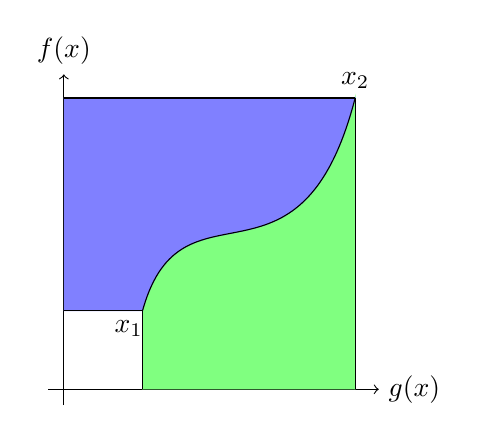
\begin{tikzpicture}
		\draw[->] (-0.2,0) -- (4,0) node[right]{$g(x)$};
		\draw[->] (0,-0.2) -- (0,4) node[above]{$f(x)$};
		\node[left=5,below](x1) at (1,1) {$x_1$};
		\node[right,above](x2) at (3.7,3.7) {$x_2$};
		\filldraw[green!50] (1,0) -- (1,1) ..controls(1.5,2.8) and (3,1) ..(3.7,3.7) -- (3.7,0);
		\filldraw[blue!50] (0,1) -- (1,1) ..controls(1.5,2.8) and (3,1) ..(3.7,3.7) -- (0,3.7);
		\draw (1,1) ..controls(1.5,2.8) and (3,1) ..(3.7,3.7);
		\draw (1,0) -- (1,1);
		\draw (0,1) -- (1,1);
		\draw (3.7,3.7) -- (3.7,0);
		\draw (3.7,3.7) -- (0,3.7);
	\end{tikzpicture} 
\end{figure}

\subsubsection{微分方程}
受迫阻尼振动:
\[m \ddot{x} = -kx-\gamma \ddot{x}+F(t)\]
Schrodinger equation:
\[i\hbar \frac{\partial \psi}{\partial t} = -\frac{\hbar^2}{2m} \frac{\partial^2 \psi}{\partial x^2}+V\psi\]

\subsubsection{卷积}
\begin{align}
k(t) = \int_{x_1}^{x_2} f(x) g(t-x) \mathrm{d}x \equiv f*g\\
(f*g)*h = f*(g*h)
\end{align}

\subsubsection{高数中难理解的问题}

\[
f(x) = \left\{
\begin{array}{lc}
e^{-\frac{1}{x^2}} & (x \neq 0)\\
0                  & (x = 0)     
\end{array}
\right.
\]

\begin{figure}
	\centering
	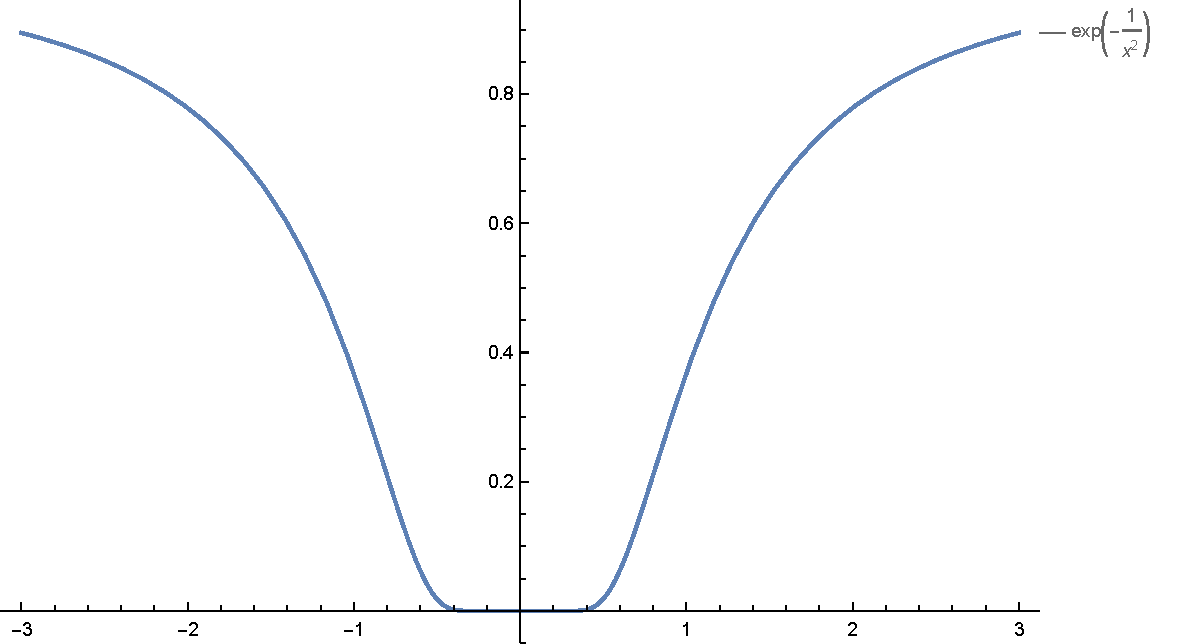
\includegraphics[width=3.95cm]{Figures/Exp[-x^-2].pdf}
\end{figure}

$f(x)$在0点光滑,$f^{(n)} = 0$,Taylor展开之后:$f(x) = 0$\\
复变函数中:
\[f(z)=e^{-\frac{1}{z^2}}\]
在$z = 0$有本性奇点,展开半径为0,故不能Taylor展开,但可以用Laurent展开。

\[f(x)=\frac{1}{1+x^2}\]
Taylor展开的收敛区域为$(-1,1)$.在复数域看:$f(z)=\frac{1}{1+z^2}$在$\pm i$为奇点!所以展开半径为1,只能在$(-1,1)$展开。




